\documentclass{msuposter}
\usepackage{lipsum}
\usepackage{tikz,wrapfig}
%% REQUIRED
\title{Using GANs to Generate Synthetic Data}
\author{Joseph Despres and Yunus Shariff}
\institute{Michigan State University}


%% SET COLUMN WIDTH
\newcommand{\colwidth}{0.3\linewidth}

\begin{document}
\begin{frame}{}
\begin{columns}[t]

\begin{column}{\colwidth}

\begin{block}{Introduction and Motivation}

This project aims to extend the Generative Adversarial Network GAN) beyond image generation by using the framework to create synthetic data. The objective of any GAN is to train a Neural Network to fit a dataset so well, that it can generate additional copies indistinguishable from the real training data. This is accomplished by training two adjacent Neural Networks, one trained to distinguish generated data from the real, while the other is trained to generate data that fools the first network\cite{NIPS2014_5ca3e9b1}. This area has shown so much progress in the past several years, today's GANs are regularly generating images and videos that can fool even the most observant humans. Applications for this technology have yet to be fully realized. This project explores a potential application of this technology. We aim to generate tabular data in a similar structure as training data however, that will be indistinguishable, yet different from real data. 

\end{block}

\begin{block}{Potential Use Cases}

\begin{itemize}
	\item \textbf{Use to generate additional datapoints in Controlled experiments}
\end{itemize}


Although data are becoming more and more available, there is still a need to generate more. First, big datasets are often convenient to collect and not controlled experiments, therefore samples in a randomized controlled trial are going to still be quite expensive. Additionally, Neural networks are not as transparent as a statistical model. We feel these are natural complements, as we are developing a framework in which Neural Networks generate additional data and statistical models could be used to draw inferences based on what the network learned.

\begin{itemize}
	\item \textbf{Use to generate data to fit models where data are confidential}
\end{itemize}

Since these data are generated as a result of what is seen on a data set confidentially and privacy is far less of a concern. This framework could be used to generate new samples of confidential data permitting models to be trained in a way that is compliant with regulatory standards, ethics, and respectful of privacy. Privacy concerns are not nearly as strong of a concern as in computer-generated data, as these are merely data produced from learning the structure of the mechanism producing the data. 



\end{block}

\begin{block}{Method}

The challenge associated with training a GAN to generate synthetic data in a row in a data frame is several orders of magnitude smaller than a standard photo image. A Neural Network has no difficulty fitting it with enough hidden layers. The challenge is learning the structure of the data without overfitting. This is a balance between fitting the data so well it mimics the data seen and underfitting where it cannot generate. Therefore, the networks are very shallow by modern standards. 


\begin{figure}
  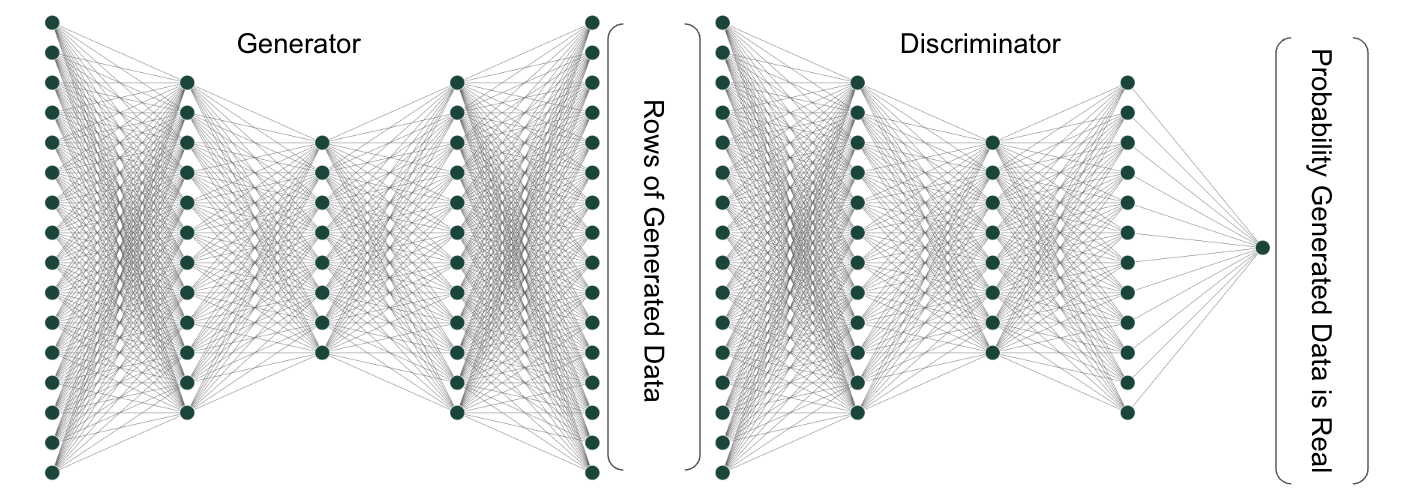
\includegraphics[width=\linewidth]{gan_diag.png}
    	\caption{\label{fig:my-label} Basic GAN Architecture Adapted to Generating Data}
\end{figure}

$$
\min_{G} \max_{D} V(D, G) = \mathop{\mathbb{E}}_{x \sim p_{data}} logD(x) + \mathop{\mathbb{E}}_{z \sim p_{z}(z)}log(1-D(G(z)))
$$

Using the method outlined by Hung \cite{hung} to generate additional data samples. These networks are small by today's standards with each layer being made up of less than 200 neurons and the network is made of less than 10 layers. Real and generated data are combined into a single data frame the discriminating network outputs a probability the data are real and fake given what it has learned from the training process. This is an iterative process and continues training until it converges to the point in which data are indistinguishable from real data. This training simply runs until all the numbers in the probability vector are 1.


\newpage 

\end{block}. 


\end{column}

%% COLUMN DIVIDE %%%%%%%%%%%%%%%%%%%%%%%%%%%%

\begin{column}{\colwidth}

\begin{block}{Experiment}

Here we will use a curated dataset to generate synthetic copies. In this project, we use New York City Taxi from 2016\cite{nyc2016}. We selected these data for ease of verification. We generate a longitude, latitude, and time of pick-up and drop-off. After that, we assemble the GAN architecture, then train a GAN on a subset of the data, then retrain adding more and more data points. See Figure 2 for a minimal example of the process of concatenating real and generated data and training a network to identify the differences. 


\begin{figure}
  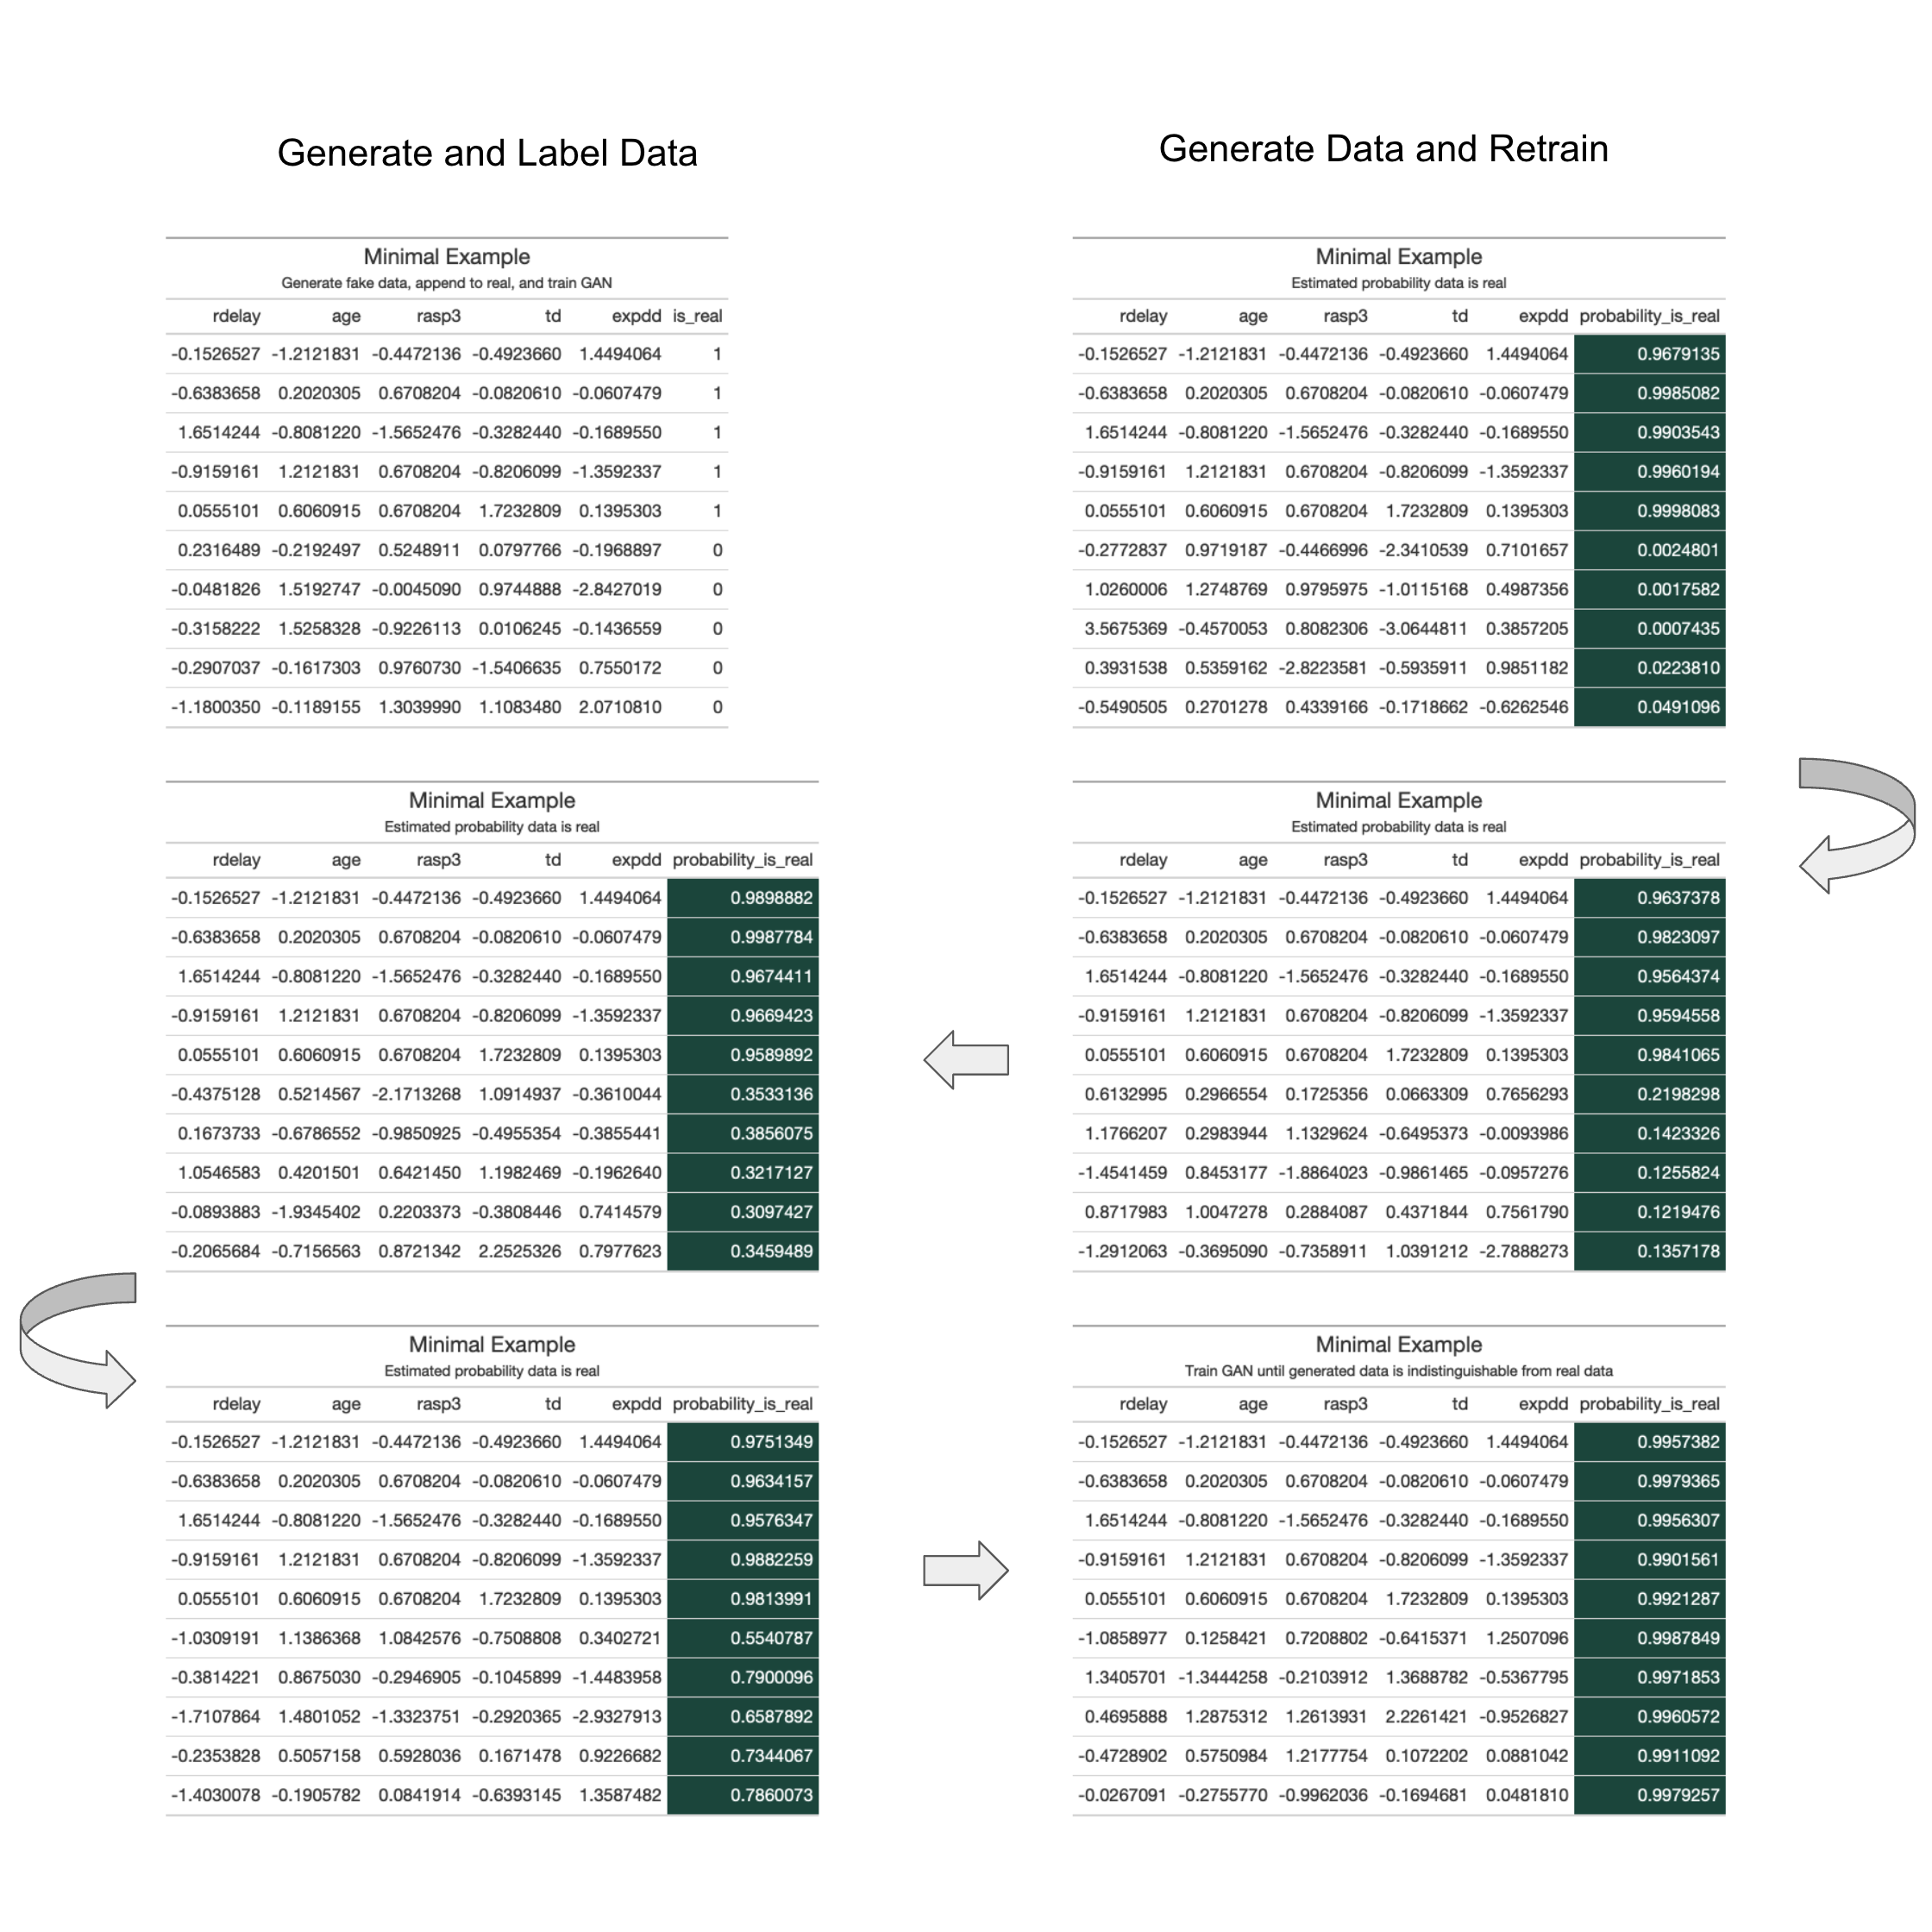
\includegraphics[width=\linewidth]{gan_conv.png}
      	\caption{\label{fig:my-label} GAN Generating Synthetic Data and Estimating Probability is Real}
\end{figure}



\begin{figure}
  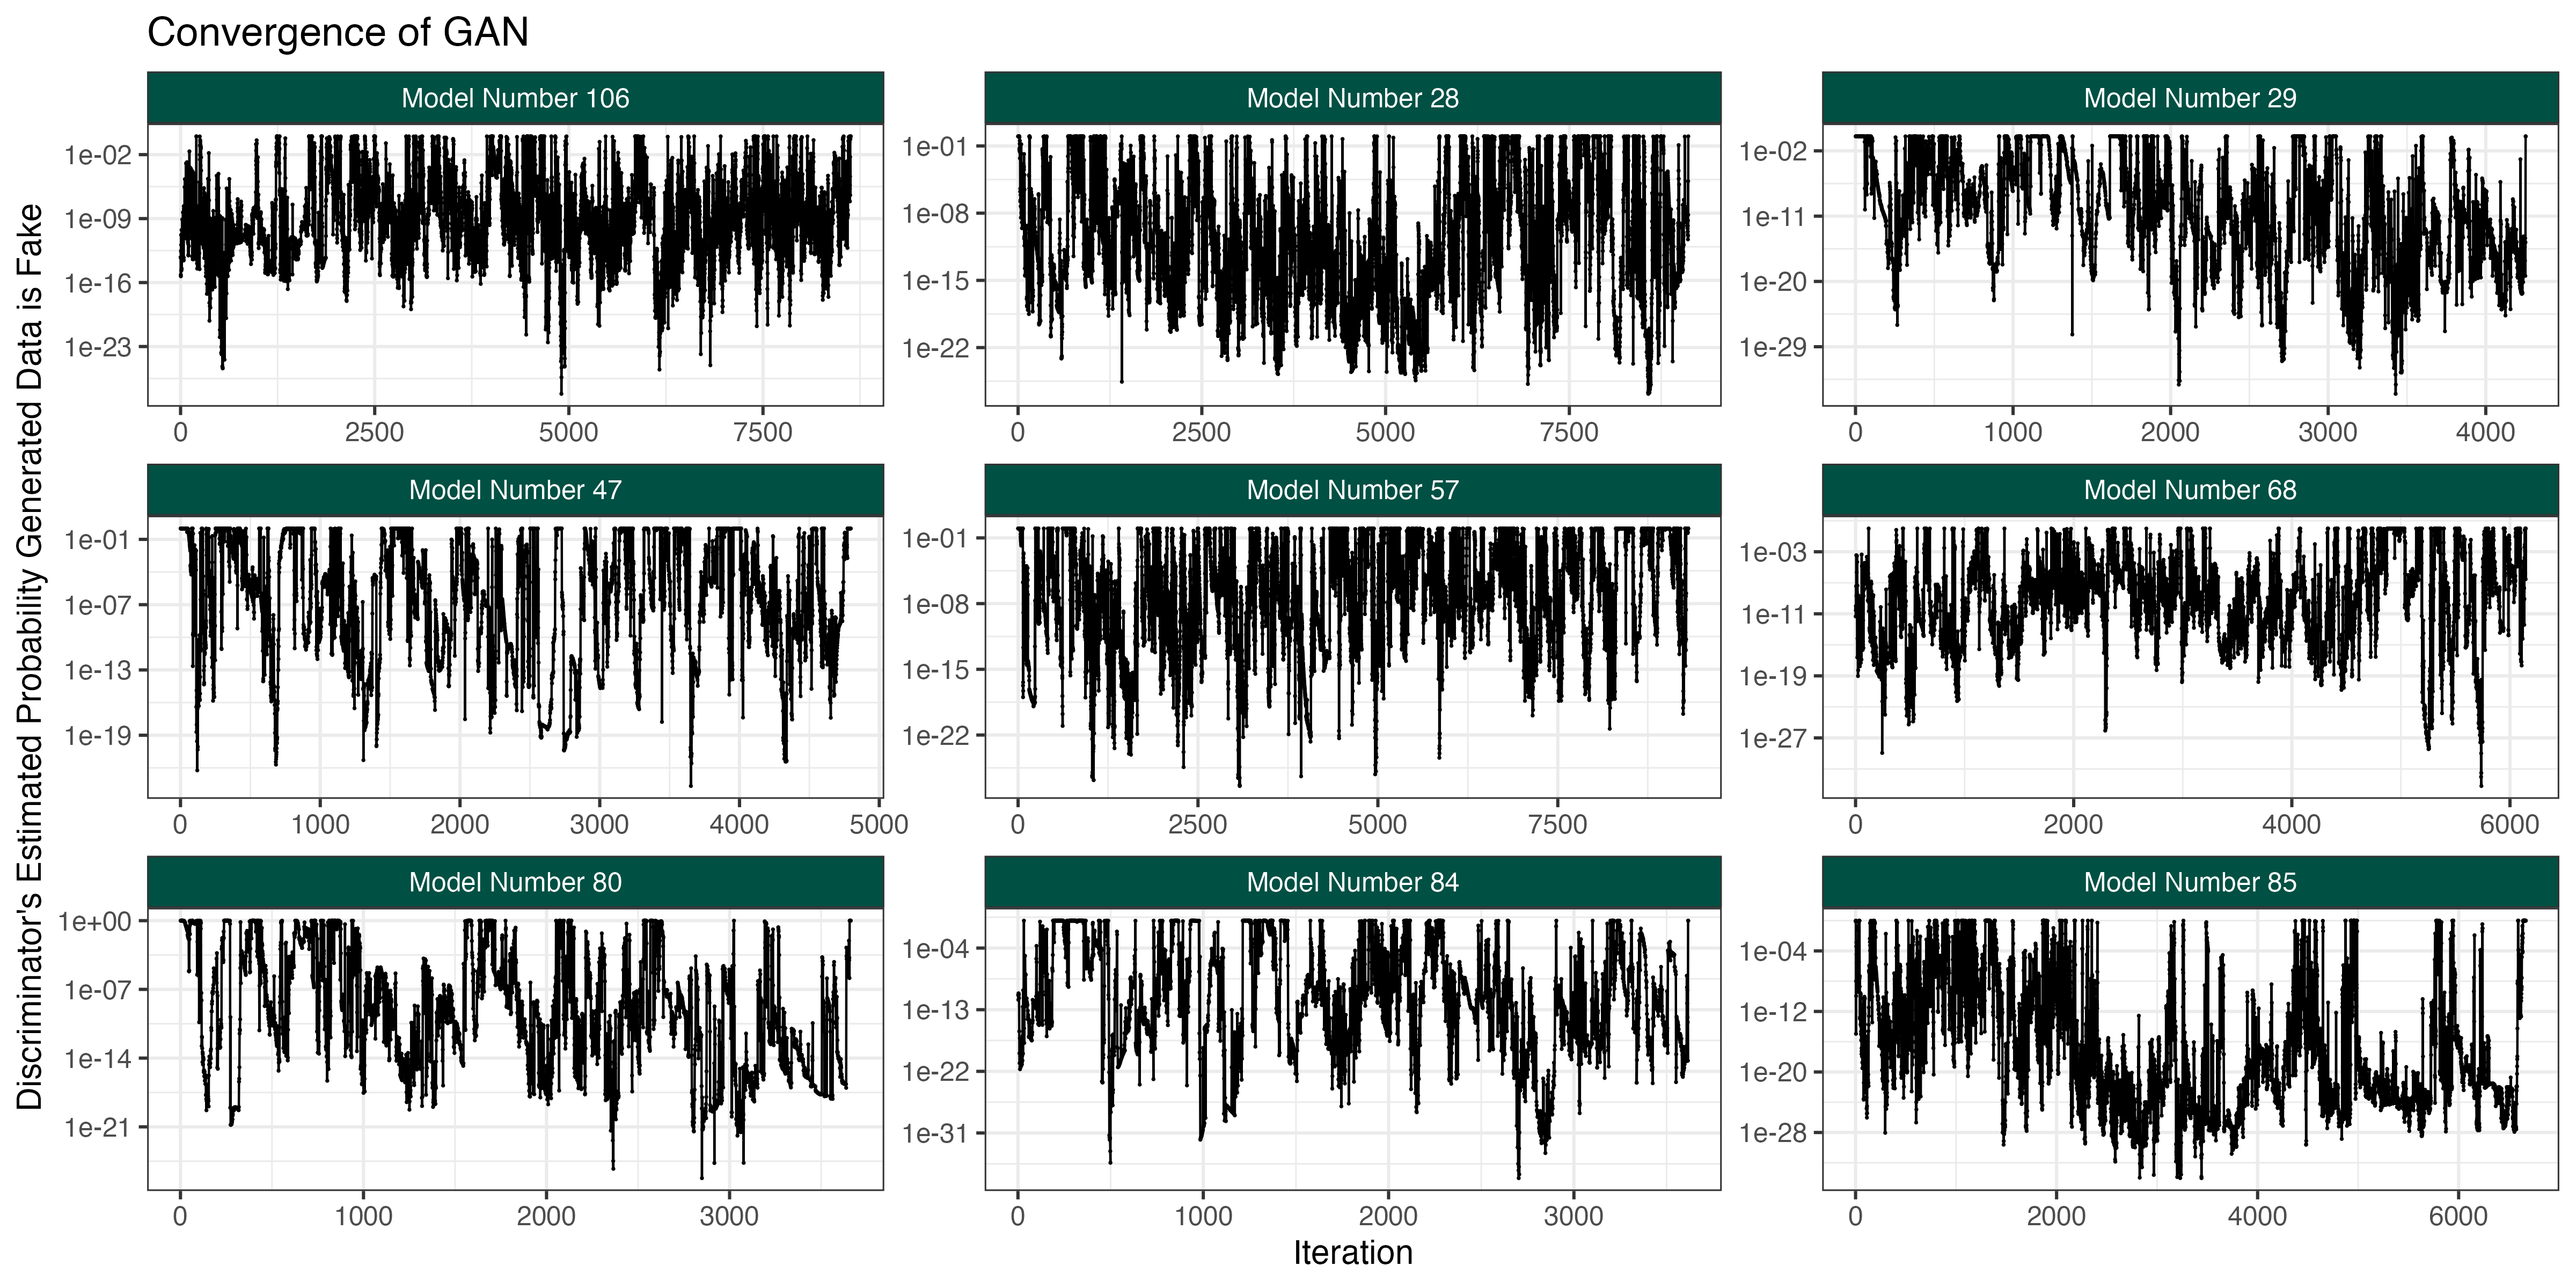
\includegraphics[width=\linewidth]{gan_converging.png}
  	\caption{\label{fig:my-label} New York City Taxi Data Real and Generated}
\end{figure}

As the GAN trains, generated data are assigned a very low probability of being real. Note in Figure 3 that the training process is cyclical where at times the generator is generating better samples than the discriminator is better at detecting generated samples. When this converges to 1, the discriminator is unable to distinguish between real and generated. 


\end{block}
\end{column}

%% COLUMN DIVIDE %%%%%%%%%%%%%%%%%%%%%%%%%%%%

\begin{column}{\colwidth}


\begin{block}{Results}

Here we were able to generate synthetic taxi rides. Notice these generated taxi rides follow a different structure from the dataset. The dataset contains a significant number of taxi rides going from the airport to midtown, where the generated samples are going from midtown tout to the surrounding borrows. These generated samples, like most GANs, do require manual curation. Taxis should not be dropping people off in the middle of the river or on expressways. We can see that happening in our generated samples. Other than that, these require significant manual inspection, which admittedly is limiting applications. 


\begin{figure}
  \includegraphics[width=\linewidth]{generated_map.png}
  	\caption{\label{fig:my-label} Probability data are real}
\end{figure}



An additional limitation of this method is the need to retrain the GANs after several different generated data points.
\end{block}


\begin{block}{Limitations and Further Study}

Despite the shallow architecture, this is quite expensive. This is because when our GANs converge they often converge to generate a single point. To remedy this, we retrain the GAN using a slightly different architecture often generating a random number of neurons. This adds variation to the system, however, it uses randomly initialized networks. Additional study would involve data verification that does not involve a visual inspection. The need for visual inspection limits the type of applications this can be useful because most data will not be easy to verify. Also, using multiple datasets as well as adding convolutions to this network. This is the beginning of what could be a helpful method. 

\end{block}

\begin{block}{References}
\scriptsize
\bibliography{references}
\bibliographystyle{plain}
% \end{scriptsize}
\end{block}

%%%% end of references %%%%%%%%%%%%%%%%
\end{column}

\end{columns}
	\end{frame}
\end{document}


